\documentclass{121Temp}

\usepackage{amsmath}
\usepackage{amssymb}
\usepackage{amsthm}
\usepackage{commath}
\usepackage{listings}
\usepackage{mathtools}
\usepackage{float}

\usepackage{hyperref}

\usepackage{graphicx}
\graphicspath{ {images/} }

\hwauthor{Jonathan Levine}{jonlevi@sas.upenn.edu}
\hwcourse{BIBB 585}
\hwrecitation{401}
\hwno{1}

% \date{}  % uncomment this line to suppress the current date in the title
% \date{Due: Never}  % or uncomment this line to manually add a date
% \hwonelateday                   % uncomment either this line or the next to
% \hwtwolatedays                  % indicate that you are using an extension

\begin{document}
\maketitle

% Problem 1
\hwproblem
\label{Q1}
Sub-threshold membrane dynamics depend on the time constant of the membrane, which is product of $r_m*c_m$, and the external current. All active conductances are ignored, and the resistance/conductance is assumed to be a constant and not a function. Thus the model, assuming sub threshold constant conductances, yields an RC circuit with a time constant depending on the input resistance and the capacitance of the membrane. Essentially, taking the current as $C_m \times \frac{dV}{dt}$, we multiply by $r_m$ to create this time constant $\tau$, which then is definitioanlly equal to $r_m \times -g_l \times (driving force) + I_ext$, which simplifies to equation 1.
% Problem 2
\hwproblem
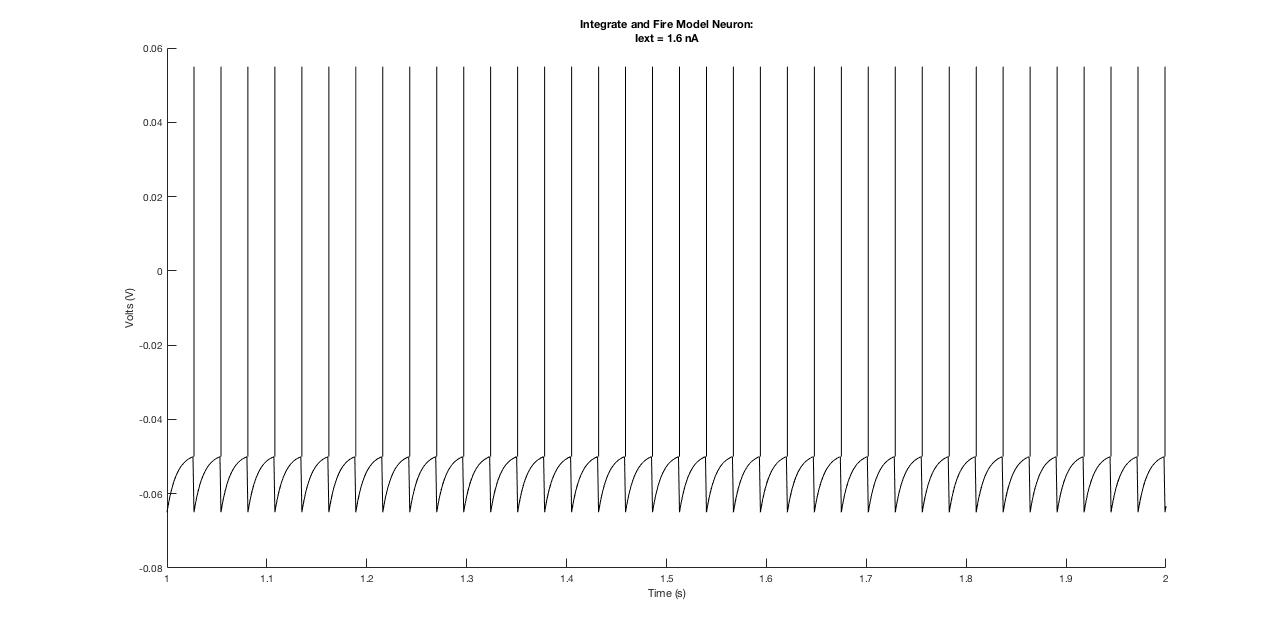
\includegraphics[scale=.45]{one.jpg}

For constant current = 1.6 nA, we can get a very regular spiking pattern. The subthreshold rise in voltage leading up to spike threshold is given by the differential equation explained above.

% Problem 3
\hwproblem
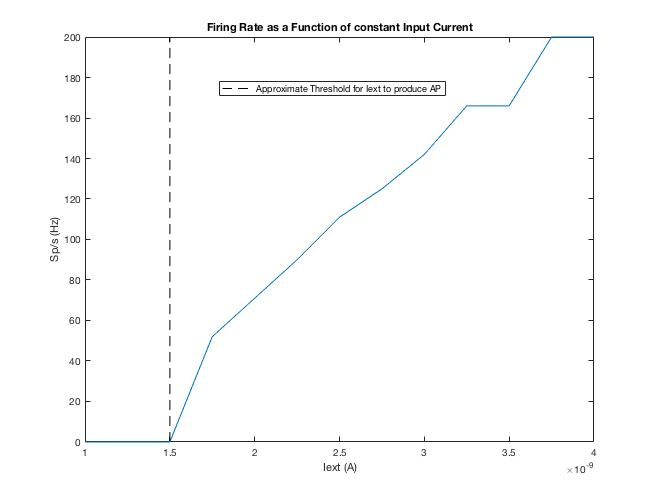
\includegraphics[scale=.75]{two.jpg}
The firing rate, in spikes/sec, depends on the input current. The higher the input current, the faster the voltage will rise to threshold and will cause a spike/reset. Below a certain level, there is not enough input current to reach threshold voltage. The approximate minimum value in order to eventually reach threshold is around 1.5 nA, as shown in the dotted line. 


% Problem 4
\hwproblem
The input current does not necessarily have to be constant. Below are three functions I(t): \\
For a sinusoidal input current, the neuron spikes in bursts corresponding to the peaks of the sine wave, and goes through waves of inhibition corresponding to the troughs.

For normally distributed current centered (mean 1.25 nA , SD 1 nA,) the neuron occasionally spikes, but mostly stays subthreshold in a noisy depolarization/hyperpolarization battle. 

For current as a downward facing parabola centerd at t = 1.5, around the vertex of the parabola we have a high spike frequency, which tapers off eventually leading to no spiking at all on the periphery.

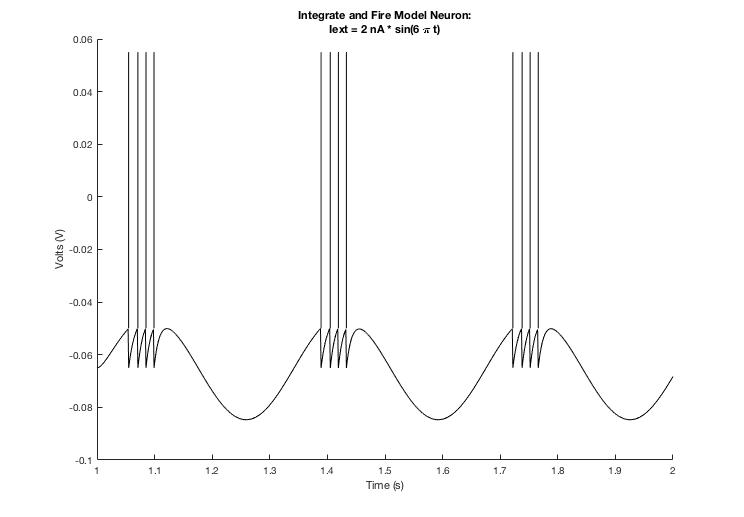
\includegraphics[scale=.65]{sine.jpg}

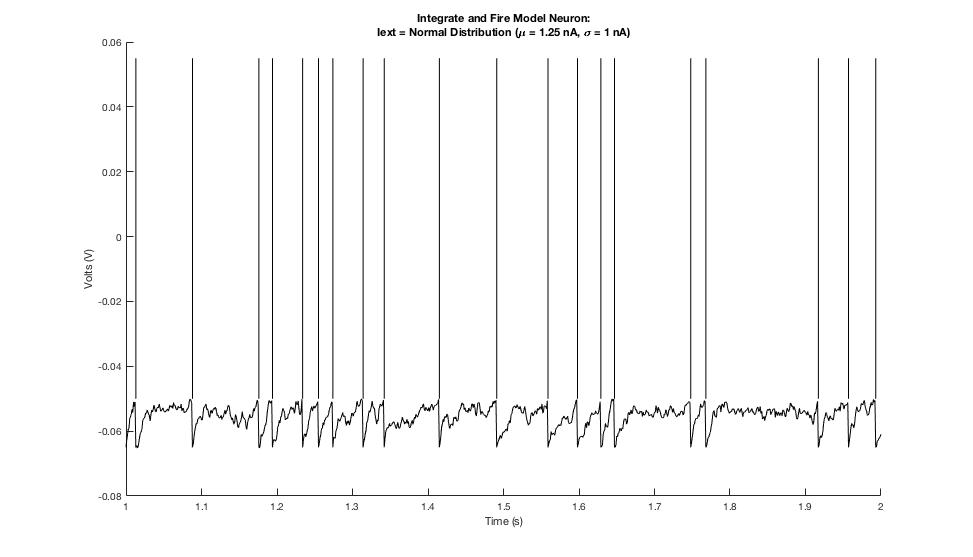
\includegraphics[scale=.55]{normrnd.jpg}

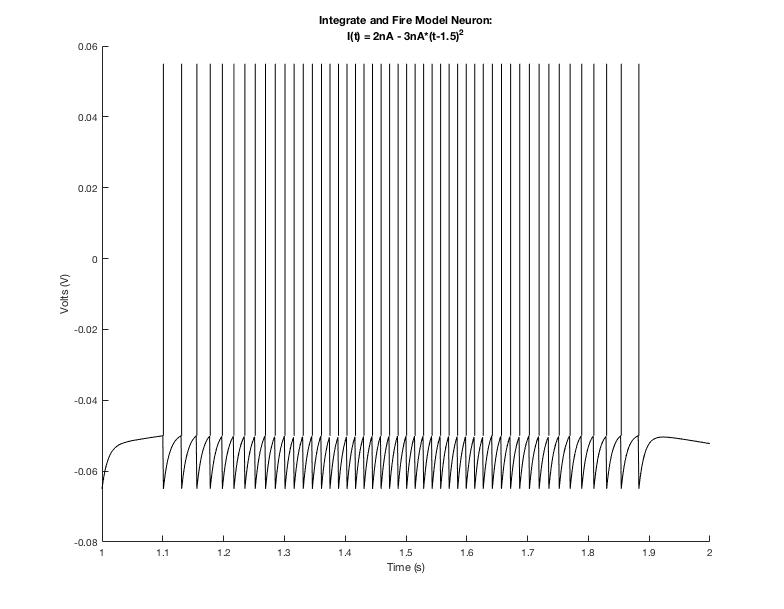
\includegraphics[scale=.55]{parabola.jpg}


\hwproblem
BONUS: \\
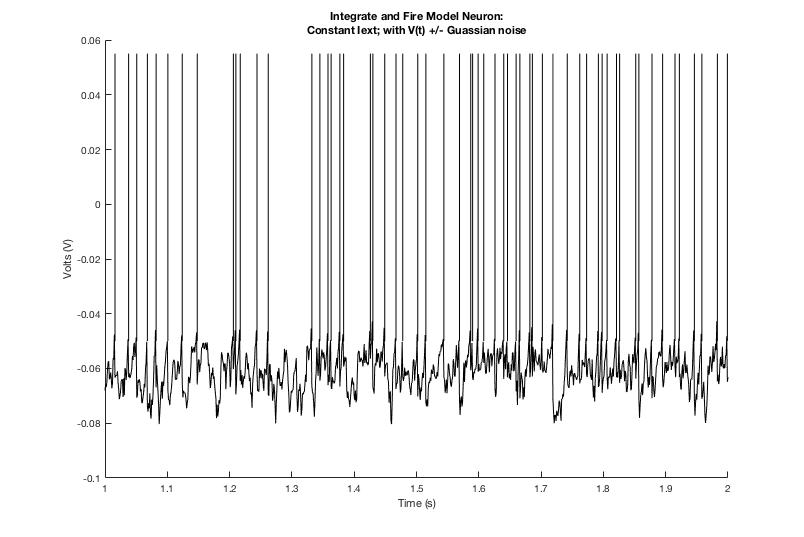
\includegraphics[scale=.55]{noisy.jpg}

The noise makes the spiking more irregular and "noisy", in that the same current does not always produce the same increase in voltage, and thus the time course for generating voltage up to threshold changes from spike to spike dictated by the random noise, creating an irregular stochastic pattern


\end{document}